\chapter{Cooper-Paare und Supraleitung\label{chapter:supraleitung}}
\lhead{Cooper-Paare und Supraleitung}
\begin{refsection}
\chapterauthor{Simon Kuster und Nicola Ochsenbein}




\newpage
%----------------------------Einleitung------------------------
\section{Einleitung}
\rhead{Einleitung}
In diesem Kapitel m"ochten wir die Grundlagen f"ur die Supraleitung erarbeiten. Ausgehend von der bekannten coulombschen Wechelwirkung zwischen Elektronen, wollen wir verstehen wie und aus welchem Grund sich Elektronen zu Paaren binden, sogenannte Cooper-Paaren. Dazu m"ussen wir zuerst den Effekt der Elektron-Elektron Wechselwirkung verstehen. Aufbauend k"onnen wir dann erkl"aren, welches die energetisch g"unstigsten und somit auch wahrscheindlichsten Konstellationen sind, unter welchen sich die Elektronen zu Paaren binden.
%TODO Auf Literatur verweisen, wie?

%----------------------------Elektron-Elektron Wechselwirkung------------------------
\section{Elektron-Elektron Wechselwirkung\label{supraleitung:elektronelektronwecheslwirkung}}
\rhead{Elektron-Elektron Wechselwirkung}
Damit sich Elektronen zu Paaren bilden, m"ussen sie sich anziehen. Die bekannte coulombsche Wechselwirkung ist jedoch abstossend. Dies liegt daran, dass die Ladungen der Elektronen die selben Vorzeichen aufweisen.
\begin{equation}
F = \frac{Q_1\cdot Q_2}{4\pi \varepsilon r^2}
\label{supraleitung:Coulomb}
\end{equation}
Wir sind also auf der Suche nach einer anziehenden Kraft. Um der Vorzeichenkonvention zu entsprechen muss die Kraft negativ sein.
\\
Zwischen den Elektronen und dem Gitter ist eine Wechselwirkung vorhanden. Diese reine Wechselwirkung zwischen Gitter und Elektron hat jedoch keinen Einfluss auf die Elektron-Elektron Wechselwirkung. Sie wird deshalb nachfolgend nicht ber"ucksichtigt.
Die f"ur uns interessante Elektron-Elektron Wechselwirkung funktioniert "uber die sogenannten Phononen. Wie diese Wechselwirkung im Allgemeinen funktioniert und was Phononen sind wird nachfolgend erl"autert.
\\
\\
In Abbildung \ref{supraleitung:Gitter1} betrachten wir einen Ausschnitt der Gitterstruktur eines K"orpers. Fliegt nun ein Elektron in dieses Gitter hinein, so wird das Gitter durch das elektrische Feld des Elektrons deformiert. Das Elektron "andert seine Flugbahn. Dargestellt ist dies in Abbildung \ref{supraleitung:Gitter2}. Das deformierte Gitter bewegt sich nun weiter als Schwingung. In Abbildung \ref{supraleitung:Gitter3} ist diese Schwingung dargestellt und mit $q$ bezeichnet. Wenn nun ein weiteres Elektron ins Gitter fliegt und auf die Schwingung trifft, so wird dieses von der Schwingung im Gitter beeinflusst, ersichtlich in Abbilung \ref{supraleitung:Gitter4}. Die Schwingung im Gitter wird wieder vernichtet und das zweite Elektron ver"andert ebenfalls seine Flugbahn. Es wurde also ein Impuls vom Elektron $k'$ zum Elektron $k$ "uber das Gitter transportiert. 
\\
\\
Die Schwingng $q$ welche vom Elektron $k'$ zum Elektron $k$ "transportiert" wurde entspricht einem harmonischen Oszillator. Nach Kapitel \ref{chapter:harmonischeroszillator} bedeuted das, dass die m"oglichen Frequenzen, und die damit die enthaltenen Energieniveaus, quantisiert sind. Wenn diese Energie quantisiert ist, kann man die Energie der Einfachheit halber als Teilchen betrachten. Diese neu eingef"uhrten Teilchen werden Phononen genannt.\\
\\
Um die Darstellung der Wechselwirkung zu vereifachen, zeichnen wir nun dieses Phonon als zickzack Vektor zwischen Elektron $k'$ und $k$. Diese Darstellung nach Feynman ist in Abbildung \ref{supraleitung:FeynmanDiagram1} ersichtlich.
\\
%TODO hier sollte auf das Feynmandiagramm verwiesen werden. (wie?)
%Kann das verhalten der Bilder so beeinflusst werden, dass sie wenigstens im gleichen unterkapitel angezeigt werden? (momentan ist die Darstellung der Bilder "uber so viele Seiten nicht geeignet.
\newcommand{\marrow}[5]{%
    \fmfcmd{style_def marrow#1
    expr p = drawarrow subpath (1/4, 3/4) of p shifted 6 #2 withpen pencircle scaled 0.4;
    label.#3(btex #4 etex, point 0.5 of p shifted 6 #2);
    enddef;}
    \fmf{marrow#1,tension=0}{#5}}
\begin{center}
\begin{fmffile}{supraleitung/phonon}
\begin{fmfgraph*}(100,60)
\fmfleftn{i}{2}
\fmfrightn{o}{2}
\fmflabel{$\vec k'-\vec q$}{i1}
\fmflabel{$\vec k'$}{i2}
\fmflabel{$\vec k+\vec q$}{o1}
\fmflabel{$\vec k$}{o2}
\fmf{fermion}{i2,v1,i1}
\fmf{fermion}{o2,v2,o1}
\fmf{zigzag,label=$\vec q$}{v1,v2}
\fmfdot{v1,v2}
\marrow{c}{up}{top}{}{v1,v2}
\end{fmfgraph*}
\qquad
\qquad
\qquad
\begin{fmfgraph*}(100,60)
\fmfleftn{i}{2}
\fmfrightn{o}{2}
\fmflabel{$\vec k'+\vec q$}{i1}
\fmflabel{$\vec k'$}{i2}
\fmflabel{$\vec k-\vec q$}{o1}
\fmflabel{$\vec k$}{o2}
\fmf{fermion}{i2,v1,i1}
\fmf{fermion}{o2,v2,o1}
\fmf{zigzag,label=$-\vec q$}{v1,v2}
\fmfdot{v1,v2}
\marrow{c}{up}{top}{}{v2,v1}
\end{fmfgraph*}
\end{fmffile}
\end{center}

Entstehung von Cooper-Paaren und Supraleitung nach Feynman
%\caption{Entstehung von Cooper-Paaren und Supraleitung nach Feynman
%\label{supraleitung:FeynmanDiagram1}}
\cite{supraleitung:feynman}.
\begin{figure}
\centering
\includegraphics[width=0.4\textwidth]{supraleitung/gitter-1.pdf} %Bild Ungestoertes Gitter
\caption{Ungest"ortes Gitter
\label{supraleitung:Gitter1}}
\end{figure}
\begin{figure}
\centering
\includegraphics[width=0.4\textwidth]{supraleitung/gitter-2.pdf} %Bild Gitter mit Elektron1
\caption{Elektron fliegt ins Gitter und st"ort dieses
\label{supraleitung:Gitter2}}
\end{figure}
\begin{figure}
\centering
\includegraphics[width=0.4\textwidth]{supraleitung/gitter-3.pdf} %Bild Gitter mit Stoerung
\caption{Gitter mit Schwingung q
\label{supraleitung:Gitter3}}
\end{figure}
\begin{figure}
\centering
\includegraphics[width=0.4\textwidth]{supraleitung/gitter-4.pdf} %Bild Gitter mit Elektron2
\caption{Elektron fliegt ins Gitter und wird beeinflusst
\label{supraleitung:Gitter4}}
\end{figure}
\\
Diese Wechselwirkung zwischen den Elektronen nur Grafisch zu betrachten reicht nicht um eine Aussage "uber die Anziehung oder Abstossung zu machen. Wir werden also nachfolgend diese Wechselwirkung mathematisch entwickeln. F"ur die mathematische Betrachtung beginnen wir da wo wir einen Anhaltspunkt haben, also beim Phonon.
\\
Wir haben gesehen, dass das Phonon einem harmonischem Oszillator entspricht und quantisiert ist. F"ur das Phonon gibt es also Auf- und Absteigeoperatoren. Wenn wir das Phonon $a$ nennen und die Energie $q$ haben, ergibt sich der Aufsteigoperator $a^+_q$ und der Absteigeoperator $a_q$. Da die vom Phonon aufgenommene Energie quantisiert ist, so muss das Elektron qunatisierte Energie aufnehmen und abgeben. Dies bedeuted, dass auch die Elektronen Auf- und Absteigeoperatoren haben. Wir nennen die Elektronen nun $c$ mit der Wellenzahl $k$. Daraus folgt, dass der Aufsteigoperator f"ur das Elektron $c^+_k$ und der Absteigeoperator $c_k$ sind.
Wir f"uhren nun noch einen Anfangszustand $|a\rangle$ (vlg. Abb. \ref{supraleitung:Gitter1}), einen Endzustand $\langle e|$ (vgl. Abb. \ref{supraleitung:Gitter4}) und einen Zwischenzustand $|z_1\rangle$ (vgl. Abb. \ref{supraleitung:Gitter3}) ein. Der Vorgang der Wechselwirkung zwischen den Elektronen kann nun so beschrieben werden (ohne Energiebetrachtung):
\begin{equation}
\langle e|c^+_{k+q} c_k a_q |z_1\rangle\langle z_1| c^+_{k'-q} c_{k'} a^+_q |a\rangle
\label{supraleitung:WechelwirkungOE}
\end{equation}
Zu beachten ist nun, dass die Leserichtung von rechts nach links ist. Es wird also vom Anfangszustand aus ein Phonon $a$ mit der Energie $q$ erzeugt, ein Elektron $c$ mit der Wellenzahl $k'$ vernichtet und ein Elektron $c$ mit der Wellenzahl $k'+q$ erzeugt, um zum Zwischenzustand $z_1$ zu gelangen.
Von diesem Zwischenzustand aus geht es weiter, indem man das Phonon $a_q$ wieder vernichtet, das Elektron $c_k$ vernichtet und ein Elektron $c^+_{k+q}$ erzeugt.
\\
\\
Als n"achstes m"ussen wir die Energiebetrachtung einf"ugen. Daf"ur f"uhren wir eine materialabh"angige Konstante $M_q$ ein und erg"anzen die Wechselwirkung mit dem Nenner aus der St"orungstheorie.
Um die gesammte Wechselwirkung zu erhalten summieren wir "uber alle $k$, $k'$ und $q$. Die Wechselwirkung erg"anzen wir zudem um einen zweiten Term der die umgekehrte Wechselwirkungs-Reihenfolge enth"alt. Dies f"uhrt dazu, dass wir sp"ater weitere Vereifachungen durchf"uhren k"onnen. Da wir aber nun die Wechselwirkung doppelt z"ahlen (wir summieren ja bereits "uber alles) teilen wir noch durch $2$.
\\
\begin{equation}
\frac{1}{2}
\sum \limits_{kk'q} |M_q|^2
\left\{
\frac
{\langle e|c^+_{k+q} c_k a_q |z_1\rangle\langle z_1| c^+_{k'-q} c_{k'} a^+_q |a\rangle }
{E(k')-E(k'-q)-\hbar\omega_q}
+
\frac
{\langle e|c^+_{k'-q} c_{k'} a_{-q}|z_1\rangle\langle z_1| c^+_{k+q} c_k a^+_{-q} |a\rangle }
{E(k)-E(k+q)-\hbar\omega_q}
\right\}
\label{supraleitung:WechelwirkungME}
\end{equation}
\\
Da $E(k')-E(k'-q) = E(k+q)-E(k)$ ist, ersetzen wir diesen Teil im Nenner des ersten Bruches.
\\
Zus"atzlich k"urzen wir die Phononen und den Zwischenzustand und packen alles ausser der reinen Wechselwirkung in einen Koeffitienten $V_{kk'q}$. Somit erhalten wir die Formel
\begin{equation}
\frac{1}{2}
\sum \limits_{kk'q} 
\langle e|V_{kk'q}c^+_{k+q}c^+_{k'-q}c_{k'}c_k|a \rangle
\label{supraleitung:WechelwirkungKurz}
\end{equation}
mit
\begin{equation}
V_{kk'q} = - |M_q|^2 \left\{
\frac{1}{\hbar\omega_q-(E(k+q)-E(k))}
+
\frac{1}{\hbar\omega_q+(E(k+q)-E(k))}
\right\}
\label{supraleitung:WechelwirkungVkk'q}
\end{equation}
Wir vereinfachen weiter mit $(a-b)\cdot (a+b) = a^2-b^2$.

\begin{equation}
V_{kk'q} =
\frac
{2|M_q|^2\hbar\omega_q}
{(E(k+q)-E(k))^2-(\hbar\omega_q)^2}
\label{supraleitung:Wechelwirkung_Vkk'q_Kurz}
\end{equation}
Das Vorzeichen von $V_{kk'q}$ entscheidet nun dar"uber, ob die Wechselwirkung anziehend oder abstossend ist.\\
Da der Z"ahler Positiv ist, wird das Vorzeichen von $(E(k+q)-E(k))^2-(\hbar\omega_q)^2$ bestimmt.

%TODO nun muss die Formel 81.2 eingefuehrt werden -> Nenner noch nachvollziehbar beschreiben.
%danach richtung 81.4 weiterziehen

%----------------------------Hinzufuegen von Elektronen zu der Fermikugel------------------------
\section{Hinzuf"ugen von Elektronen zu der Fermikugel}
\rhead{Hinzuf"ugen von Elektronen zu der Fermikugel}
Angenommen, solch eine Elektron-Elektron Wechselwirkung, wie im Kapitel \ref{supraleitung:elektronelektronwecheslwirkung} beschrieben kommt zustand. Doch welche Bedingungen m"ussen erf"ullt sein?
\\
Unser Ziel wird nun sein, zwei Elektronen energetisch m"oglichst g"unstig zur Fermikugel hinzuzuf"ugen. Dazu ben"otigen wir die theoretischen Grundlagen zur Fermikugel welche im Kapitel \ref{chapter:festkoerper} behandelt sind.
\\
\\
Die Wechselwirkung zwischen den Elektronen besteht einerseits aus der altbekannten Coulombsche Wechselwirkung (\ref{supraleitung:Coulomb}) und der neu eingef"uhrten Elektronen-Elektronen Wechselwirkung. Welcher dieser Kr"afte "uberwiegt, entscheidet die St"arke der Elektron-Phononen-Kopplung.
\\
Um diese neue Wechselwirkung zu betrachten gehen wir von einem idealisierten Falls aus. Dazu kann das Modell des Elektronengases verwendet werden. Dabei sind die Valenzelektronen nicht an die einzelnen Atome gebunden sondern k"onnen sich, wie in einem klassischen Gas, frei bewegen. Diese freien Elektronen k"onnen als Leitf"ahigkeit intepretiert werden. Der Widerstand entspricht der Wechelwirkung zwischen Elektron-Gitter und Elektron-Phonon.
%TODO Klaeren ob Leitfaehigkeit und Widerstand so korrekt ist. Noch genauer recherchieren.
\\
\\
Wir betrachten die Fermikugel in der $k$-Ebene, in welcher alle inneren Zust"ande besetzt sind, alle "ausseren Zust"ande seien frei. Zu diesem System werden nun zwei Elektronen $(k_1,E(k_1))$ und $(k_2,E(k_2))$ hinzugef"ugt. Wir beschr"anken uns auf die Wechselwirkungen in welchen keine Energie an das Atomgitter abgegeben wird. Zudem beschr"anken wird die zul"assige Wechselwirkung zwischen den Elektronen auf die Energie eines Phonons.

\begin{equation}
|E(k+q)-E(k)|\le\hbar\omega_q
\label{supraleitung:Phonon Energie}
\end{equation}

\subsubsection{Wellenfunktion}
\rhead{Wellenfunktion}
Die Wellenfunktion des Elektronenpaares wir durch die Anwendung zweier Erzeugnisoperatoren auf den Grundzustand $|G\rangle$ der gef"ullten Fermikugel aufgebaut, indem wir "uber alle m"oglichen $k_1$ und $k_2$ $(|k_i| \ge k_f)$ und "uber die Elektronenspins summieren.

\begin{equation}
\Psi_{12}=\sum \limits_{k_1k_2\sigma_1\sigma_2} a_{\sigma_1\sigma_2}(k_1,k_2)c^+_{k_1\sigma_1}c^+_{k_2\sigma_2}|G\rangle
\label{supraleitung:WellenfktAllg}
\end{equation}

Um einen Zustand mit definiertem Gesamtimpuls zu erhalten, f"uhren wir die Summation in (\ref{supraleitung:WellenfktAllg}) unter der Nebenbedingung $K=k_1+k_2=const$ aus. Zus"atzlich fordern wir, dass eine Wechselwirkung zwischen den Elektronen nur dann bestehen soll, wenn sich ihre Zust"ande ausserhalb der Fermikugel mit den Energie $(E_F \le E(k_i) \le E_F+\hbar\omega_q)$ befinden.
Zusammengefasst ergeben sich folgende drei Bedingungen:
\[
\overrightarrow{k_1}+\overrightarrow{k_2}=\overrightarrow{K}=const
\]
\[
E_F\le|\overrightarrow{k_1}|\le E_F+\hbar\omega_q
\]
\[
E_F\le|\overrightarrow{k_2}|\le E_F+\hbar\omega_q
\]
%TODO Mit Titelgebung noch nicht gluecklich
\subsubsection{Optimaler Gesamtimpuls von $k_1$ und $k_2$ finden}
\rhead{Optimaler Gesamtimpuls von k1 und k2 finden}
%TODO loeschen?
%Das n"achste Ziel wird nun sein, die Elektron-Elektron Wechelwirkungsenergie zu maximieren und die dafuer notwendigen Bedingungen zu erarbeiten.
Die Wechselwirkungsenergie wird umso gr"osser, je mehr Summationsglieder zur Wellenfunktion (\ref{supraleitung:WellenfktAllg}) beitragen. Der Gesamtimpuls $K$ soll nun also so bestimmen werden, dass die Wechselwirkungsenergie maximal wird.
\\
Zur Bestimmung des optimalen $K$ kann die Fermikugel mit einer Schale der Dicke $\hbar\omega_q$ im $k$-Raum aufgezeichnet werden. In der Abbildung \ref{supraleitung:kRaum_05} wurde ein beliebiges $K$ gew"ahlt und durch geometrische Konstruktion gezeigt, in welchen Bereichen (grau markiert) m"ogliche $k_1$ und $k_2$ gew"ahlt werden k"onnen. Die graue Fl"ache entspricht der Wahrscheindlichkeit, denn je weniger Energie ben"otigt wird desto gr"osser ist die Wahrscheindlichkeit und entsprechend die graue Fl"ache. Ist $K$ gr"osser als $2\cdot(E_F+\hbar\omega_q)$ k"onnen keine g"ultigen L"osungen mehr f"ur $k_1$ und $k_2$ gefunden werden (Abbildung \ref{supraleitung:kRaum_06}). W"ahlt man hingegen $K$ kleiner und im Extremfall $K=0$ erzielt man die gr"osst m"ogliche Fl"ache und entsprechend die gr"osste Wahrscheindlichkeit (Abbildung \ref{supraleitung:kRaum_09}). Man findet also heraus, dass die Wellenzahlvektoren $k_1$ und $k_2$ entgegengesetzt sind.
\\
% Visualisierung der besten K-Vektors
% Visualisierung 1
\begin{figure}	
\centering
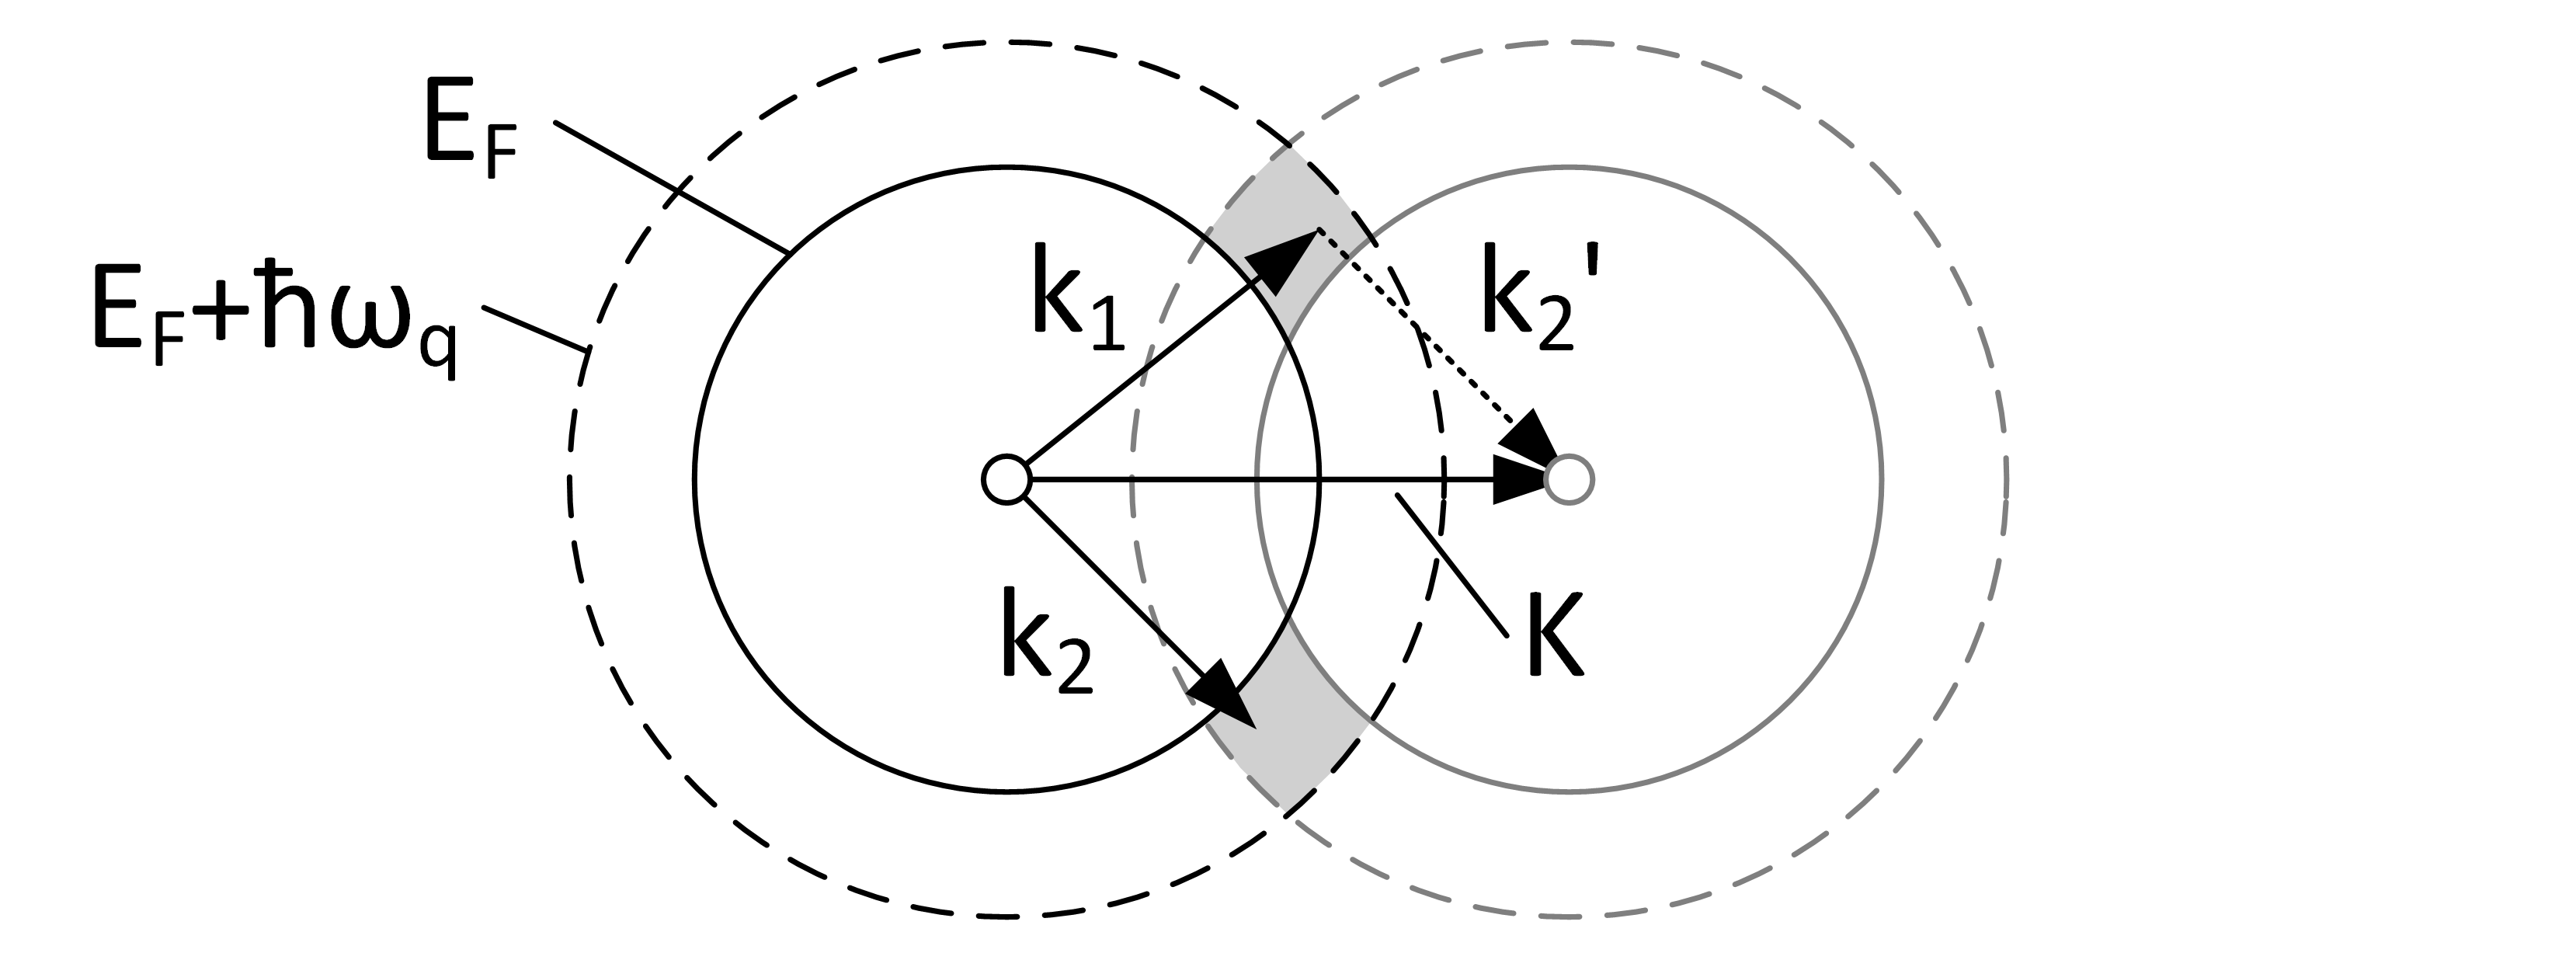
\includegraphics[width=0.6\textwidth]{supraleitung/kGraphic_05.png} %K gr"osser 0, kleiner Ef+hwq, mit Fl"achenmarkierung
\caption{beliebiges K gew"ahlt
\label{supraleitung:kRaum_05}}
\end{figure}
% Visualisierung 2
\begin{figure}	
\centering
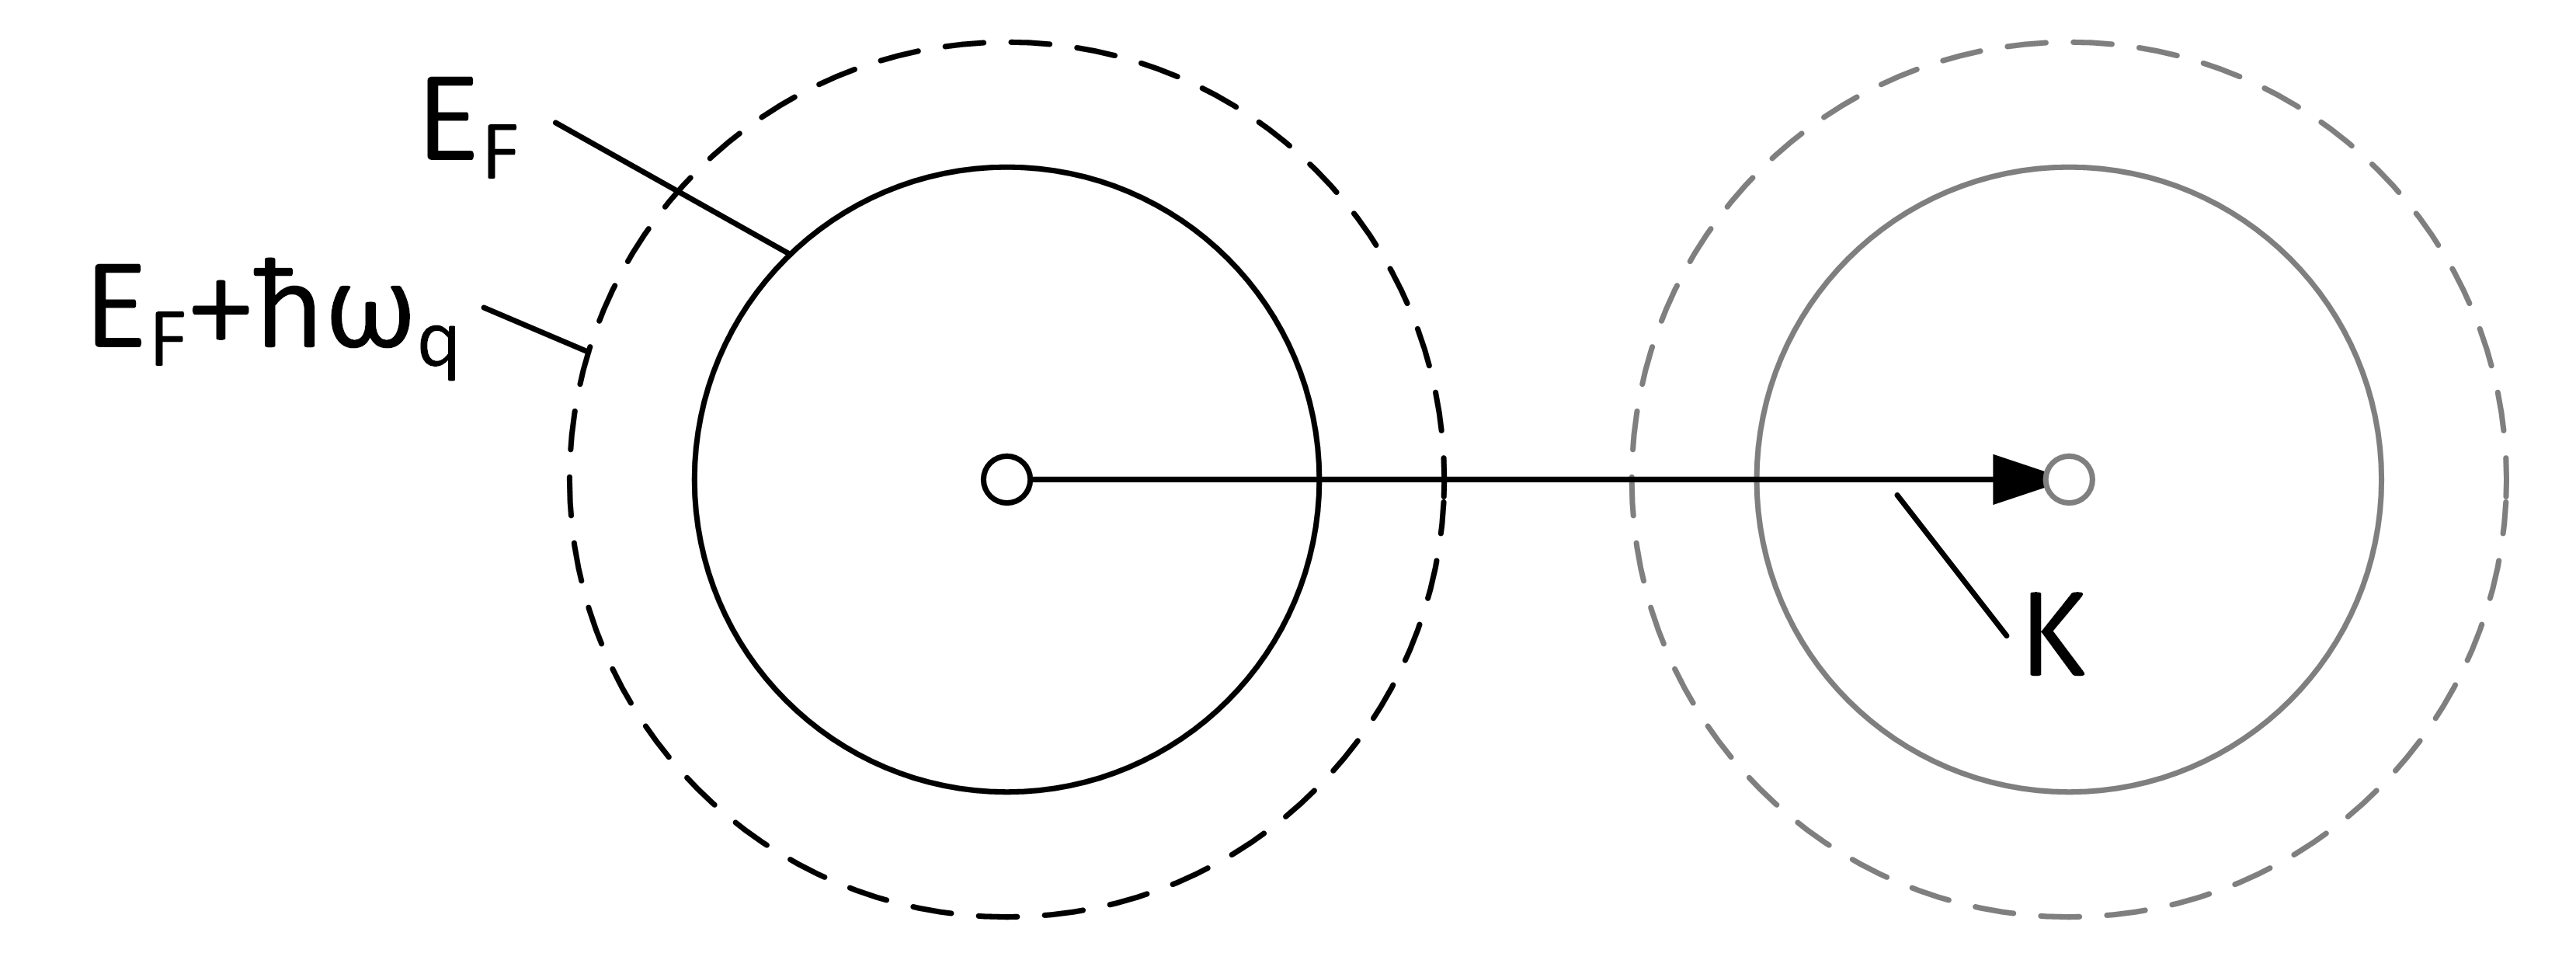
\includegraphics[width=0.6\textwidth]{supraleitung/kGraphic_06.png} %K gleich 0, mit Fl"achenmarkierung
\caption{K zu gross gew"ahlt
\label{supraleitung:kRaum_06}}
\end{figure}
% Visualisierung 3
\begin{figure}	
\centering
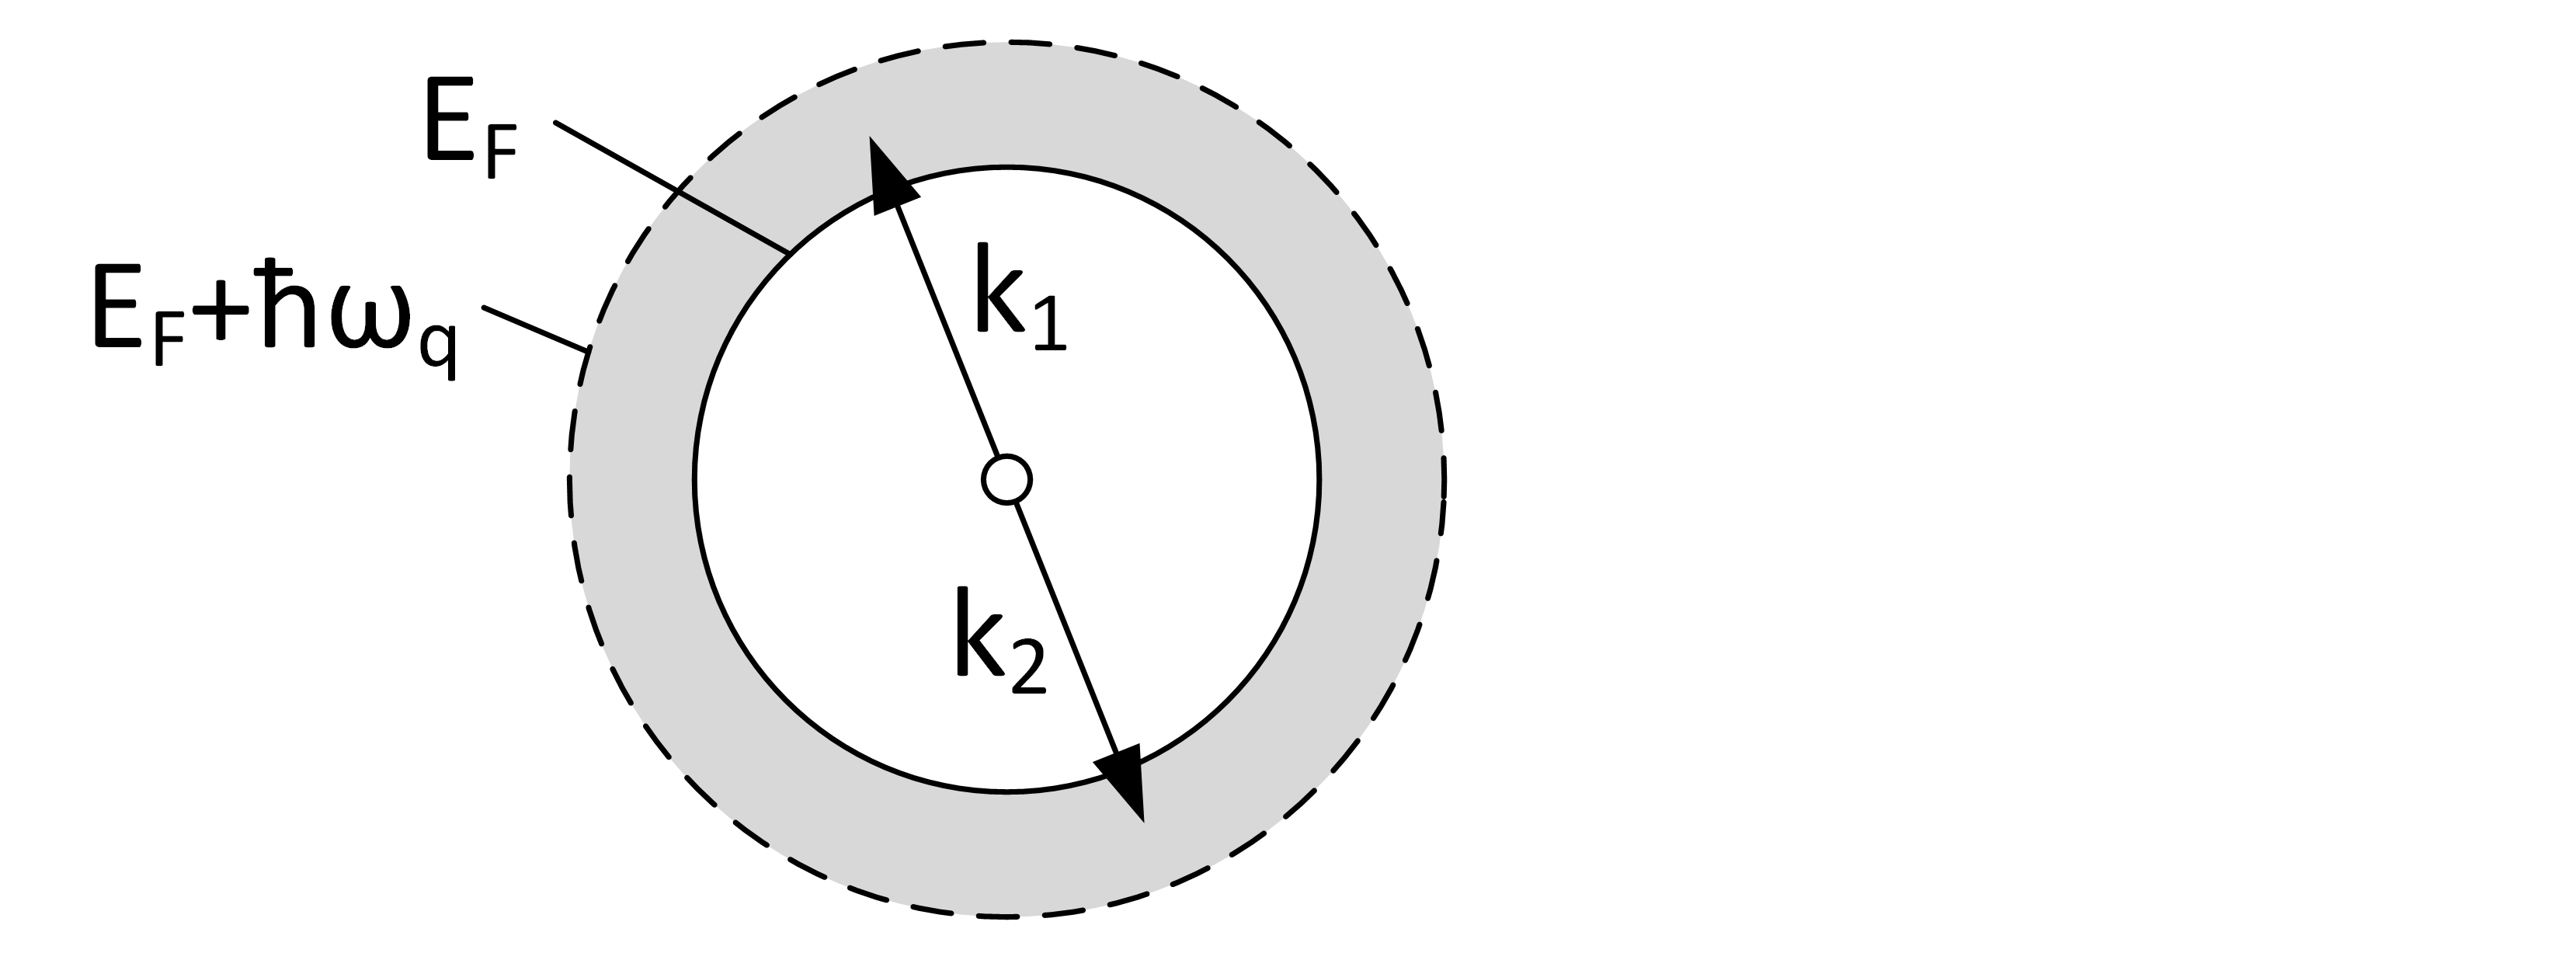
\includegraphics[width=0.6\textwidth]{supraleitung/kGraphic_09.png} %K gleich 0, mit Fl"achenmarkierung
\caption{Maximale Anzahl M"oglichkeiten um $k_1$, $k_2$ zu w"ahlen
\label{supraleitung:kRaum_09}}
\end{figure}

\subsubsection{Spin}
\rhead{Spin}
Bekanntlich besitzen Elektronen einen Spin. Da wir auf der Suche nach der maximalen anziehenden Wechselwirkung sind, nehmen wir den Elektronenspin antiparallel an. Hierzu kann die "Uberlegung mit dem entstehenden magnetischen Feld herbeigezogen werden. W"aren die Elektronenspin parallel w"urden sich die entstehenden magnetischen Felder abstossen. Wobei hingegen bei antiparallelem Elektronenspin die Wechselwirkungsenergie durch die anziehenden magnetischen Felder verst"arkt wird.

\subsubsection{Neue Wellenfunktion}
\rhead{Neue Wellenfunktion}
Mit den gewonnenen Erkenntnissen, dass $K=0$ ist und die Elektronenspins $antiparallel$, ergibt sich die vereinfachte Wellenfunktion

\[
\Psi_{12}=\sum \limits_{k} a(k)c^+_{k}c^+_{-k}|G\rangle.
\]

Um eine kompakte Schreibweise zu erhalten ordnen wir $k$ zugleich „Spin aufw"arts“ und $–k$ „Spin abw"arts“ zu. Der g"unstigste Prozess ist also wenn die Elektronen entgegengesetzte Wellenzahlvektoren $(k_1 = -k_2)$ und entgegengesetzten Spin $(\sigma_1 = -\sigma_2)$ aufweisen.
\\
%\section{Elektronenverhalten in einem Festk"orper}
%\rhead{Elektronenverhalten in einem Festk"orper}
\\

\section{Ausblick}
\rhead{Ausblick}
Wir haben also gesehen, dass es eine Elektron-Elektron Wechselwirkung gibt und wie diese zustande kommt. Das Vorzeichen und somit die Paarbildung sind aber noch nicht gekl"art. Um das Vorzeichen zu berechnen sind weiter Vereinfachungen zu treffen. Man erh"alt dann eine Gleichung mit einer zu minimierenden Nebenbedingung. Durch weitere Approximationen findet man heraus, dass 2 Elektronen als Paar weniger Energie alls alleine ben"otigen. Für die Bereichnung und als weiterführende Literatur verweisen wir auf O.Madelung Festk"orper II (\cite{skript:madelung1}).


\printbibliography[heading=subbibliography]
\end{refsection}



